\chapter{Érysichthon à jamais affamé}
\label{chap:erysichtonUsage}

intro


\section{Planification et préparations}

Nous avons nos spécificités techniques et nous savons qu'elle forme notre outil doit avoir (fig \ref{fig:compilation_structure}). Nous pouvons commencer par synthétiser les opérations nécessaires.\smallbreak

Nous allons donc concevoir des protocoles pour identifier les étapes nécessaires pour que Binsec analyse entièrement un fichier et nous renvoie un parmi [\texttt{secure, unknown, insecure}]. Le protocole \texttt{x86\_64} est particulier. Depuis la version \textbf{0.5.0} de Binsec il est possible de fournir un <<cliché mémoire>>\footnote{Plus couramment 'Core dump', terme technique anglais désignant une copie de la mémoire vive et des registres d'un programme. Ce fichier sert à être analyser, généralement par un débogueur.} pour accélérer l'analyse. Nous utilisons cet avantage pour l'intégrer à notre graphe d'éxécution.La machine sur laquelle le projet sera développé est sur une architecture x86\_64, cela nous permet d'utiliser l'outil GDB pour la génération de cliché mémoire.\medbreak

\begin{figure}[!ht]
    \caption{Protocole pour analyser des fichiers compiler en x86\_64}
    \label{fig:protocole_x86}
    \centering
  \begin{tikzpicture}[auto]

    % Styles
    \tikzstyle{startstop} = [rectangle, rounded corners, minimum width=2cm, minimum height=1cm, text centered, draw=black, fill=green!30]
    \tikzstyle{process} = [rectangle, minimum width=2cm, minimum height=1cm, text centered, draw=black, fill=orange!30]
    \tikzstyle{arrow} = [thick,->,>=stealth]
    \tikzset{zone1/.style={rectangle, rounded corners, draw=red, dashed, fill=red!10, inner sep=0.3cm}}
    \tikzset{zone2/.style={rectangle, rounded corners, draw=blue, dashed, fill=blue!10, inner sep=0.3cm, opacity = 0.7}}
    \tikzset{zone22/.style={rectangle, rounded corners, draw=none, fill=blue!10, inner sep=0.3cm}}
    \tikzset{zone3/.style={rectangle, rounded corners, draw=green, dashed, fill=green!10, inner sep=0.3cm}}
    
    % Noeuds
    \node (hacl) [startstop] {Hacl*};
    \node (c) [below of=hacl] {Fonction};
    \node (ini) [below of=c, xshift=2cm] {.ini};
    \node (test) [below of=c, xshift=-2cm] {-test.c};
    \node (script) [below of=c] {.script};
    \node (compilateur) [process, below of=test] {Compilateur};
    \node (exe) [below of=compilateur] {-test.exe};
    \node (blanc1) [below of=script] {};
    \node (blanc2) [below of=blanc1] {};
    \node (gdb) [process, below of=blanc2] {GDB};
    \node (snap) [right of=gdb, xshift=2cm] {.snapshot};
    \node (binsec) [startstop, right of=snap, xshift=1.5cm] {Binsec};
    
    % Flèches
    \draw [arrow] (hacl) -- (c);
    \draw [arrow] (c) -- (ini);
    \draw [arrow] (c) -- (test);
    \draw [arrow] (c) -- (script);
    \draw [arrow] (test) -- (compilateur);
    \draw [arrow] (compilateur) -- (exe);
    \draw [arrow] (exe) -- (gdb);
    \draw [arrow] (script) -- (gdb);
    \draw [arrow] (gdb) -- (snap);
    \draw [arrow] (snap) -- (binsec);
    \draw [arrow] (ini) -- (binsec);

    % Zones
    \begin{scope}[on background layer]
        \node [zone1, fit=(c) (ini) (test) (script)] {};
        \node [zone2, fit=(script) (gdb)] {};
              \node [zone2, fit=(gdb) (snap) (binsec)] {};
              \draw [zone22]
              ([xshift=-10pt, yshift=10pt]gdb.north west) --
              ([xshift=10pt, yshift=10pt]gdb.north east) -- 
              ([xshift=10pt, yshift=-9pt]gdb.south east) -- 
              ([xshift=1pt, yshift=-1pt]gdb.south west) --
              cycle;  
    \node [zone3, fit=(compilateur) (exe)] {};
    \end{scope}
    \end{tikzpicture}
\end{figure}

Ce graphe modélise la chaîne d'étapes nécessaire à l'obtention d'une analyse Binsec pour une fonction que nous ciblons. Plusieurs zones sont distinguées. La zone verte correspond à l'étape de compilation, la zone bleue à l'étape de préparation de l'analyse et la zone rouge à la synthèse de fichiers (de tests et d'instruction pour l'analyse de Binsec). Ce choix de couleur est adapté à la difficulté attendu de chaque étape. L'opération de compilation consiste en une commande. L'opération de préparation d'analyse consiste aussi en deux commandes : un appel à GDB avec le binaire puis un appel à Binsec avec le cliché mémoire et les instruction d'analyse.\smallbreak

Avec ce graphe réalisé, nous pouvons le modifier pour préparer la voie à d'autres architectures. Dans un format plus générique voici comment se présente le protocole d'analyse :

\begin{figure}[!ht]
    \caption{Protocole générique d'analyse}
    \label{fig:protocole_generique}
    \centering
  \begin{tikzpicture}[auto]

    % Styles
    \tikzstyle{startstop} = [rectangle, rounded corners, minimum width=2cm, minimum height=1cm, text centered, draw=black, fill=green!30]
    \tikzstyle{process} = [rectangle, minimum width=2cm, minimum height=1cm, text centered, draw=black, fill=orange!30]
    \tikzstyle{arrow} = [thick,->,>=stealth]
    \tikzset{zone1/.style={rectangle, rounded corners, draw=red, dashed, fill=red!10, inner sep=0.3cm}}
    \tikzset{zone2/.style={rectangle, rounded corners, draw=blue, dashed, fill=blue!10, inner sep=0.3cm, opacity = 0.5}}
    \tikzset{zone3/.style={rectangle, rounded corners, draw=green, dashed, fill=green!10, inner sep=0.3cm}}
    
    % Noeuds
    \node (hacl) [startstop] {Hacl*};
    \node (c) [below of=hacl] {Fonction};
    \node (ini) [below of=c] {.ini};
    \node (test) [below of=c, xshift=-2cm] {-test.c};
    \node (compilateur) [process, below of=test] {Compilateur};
    \node (exe) [below of=compilateur] {-test.exe};
    \node (blanc) [below of=c] {};
    \node (blanc1) [below of=blanc] {};
    \node (blanc2) [below of=blanc1] {};
    \node (binsec) [startstop, below of=blanc2] {Binsec};
    
    % Flèches
    \draw [arrow] (hacl) -- (c);
    \draw [arrow] (c) -- (ini);
    \draw [arrow] (c) -- (test);
    \draw [arrow] (test) -- (compilateur);
    \draw [arrow] (compilateur) -- (exe);
    \draw [arrow] (exe) -- (binsec);
    \draw [arrow] (ini) -- (binsec);

    % Zones
    \begin{scope}[on background layer]
        \node [zone1, fit=(c) (ini) (test) ] {};
        \node [zone2, fit=(ini) (binsec)] {};
        \node [zone3, fit=(compilateur) (exe)] {};
    \end{scope}    
    \end{tikzpicture}
\end{figure}

Dans ce contexte, une question se pose : est-ce que la conception des scripts pour Binsec (\textit{.ini}) est automatisable ou est-ce qu'il faudra utiliser des émulateurs pour générer des clichés mémoire et revenir dans le cas de la figure \ref{fig:protocole_x86} ?\smallbreak

En effet, l'importance de cette question se révèle lorsqu'on change d'architecture et que l'on doivent se passer de clichés mémoire. Sur notre machine en x86\_64, si nous analysons un fichier compilé en ARM, alors on peut croiser des appels à des fonctions systèmes, les \texttt{IFUNC}. Or la résolution de ces fonctions est gérée dynamiquement lors de l'exécution du programme. Cette mécanique permet d'utiliser des implémentations optimisées en fonction des configurations du système d'éxécution. Or comme Binsec réalise une analyse symbolique du programme, il faut lui spécifier qu'elles fonctions correspondent aux \texttt{IFUNC} qu'il peut croiser. pour illustrer ce point, observons le scipt nécessaire pour une vérification de la fonction <<Hacl \_AEAD \_Chacha20Poly1305\_Simd128\_encrypt>> compilé vers ARMv8.

\begin{listing}[!ht]
    \caption{Script d'instruction pour analyser un binaire compilé vers ARM}
    \label{lst:script_arm_exemple}
    \begin{minted}{bash}
load sections .plt, .text, .rodata, .data, .got, .got.plt, .bss from file

secret global input1, aad1

@[0x00000048f008 ,8] := <__memcpy_generic>
@[0x00000048f018, 8] := <__memset_generic>
@[0x00000048f030 ,8] := <__memcpy_thunderx2>

starting from <main>
with concrete stack pointer


halt at <exit>
explore all 
    \end{minted}
\end{listing}

Les lignes 5 à 7 sont présentes pour indiquer les branchements à effectuer par Binsec lorsque qu'il rencontre ces adresses. Cette opération automatiquement exécutée lors de l'initialisation de l'exécution doit ici être précisée avec les fonctions présentes dans le binaire. Automatiser ces affectations peut être difficile et nécessiter quelques outils d'analyse supplémentaires pour attraper les adresses qui ont besoin d'être réaffecté et leur attribuer les fonctions les plus adaptées.\medbreak


\begin{CitationBox}{Nommer un outil}
    Rapidement il a fallu trouver un nom pour ce projet, l'appeler par "Notre outil\dots" devenait lourd et redondant entre les réunion hebdomadaire. En revanche trouver LE nom adéquat n'est pas une chose aisée, il peut être dû à une blague, une référence ou plus simplement liés au sens du projet. Dans notre cas, on aime la mythologie et le travail réalisé peut se résumer à "faut donner à manger à Binsec".\smallbreak
    Érysichthon est une personnage de la mythologie grecque condamné à être affamé au point de se dévorer lui-même pour avoir détruit l'idole d'un dieu. Ce nom me plaît et sera retenu pour la suite du projet. 
\end{CitationBox}

\subsection*{Conception d'Érysichthon}


Nous avons vus les protocoles nécessaires pour construire une analyse complète. Nous avons fait des tests pour comprendre le fonctionnement de Binsec et comment doivent être déclarer les fonctions de Hacl*. Nous passons donc en phase de conception et construisons notre outil \textit{Érysichthon}. Il sera une combinaison de script python, script shell et de Makefile. Nous appelons module un ensemble de script qui réalise une tâche au sein d'\textit{Érysichthon}. Nous vous présentons en figure \ref{fig:erysichthon} comment s'organise les modules et les tâches qu'ils effectuent.

\begin{figure}[!ht]
    \caption{Structure des modules d'Érysichthon}
    \label{fig:erysichton}
    \centering
    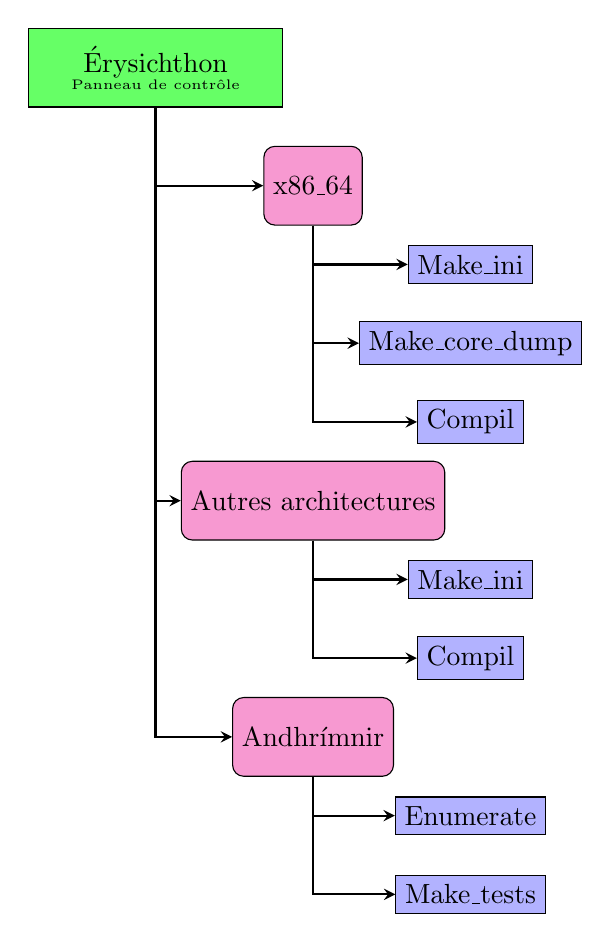
\begin{tikzpicture}[auto]

    % Styles
    \tikzstyle{startstop} = [rectangle, minimum width=2cm, minimum height=1cm, text centered, draw=black, fill=green!60]
    \tikzstyle{process} = [rectangle, rounded corners,minimum width=1cm, minimum height=1cm, text centered, draw=black, fill=magenta!40]
     \tikzstyle{process2} = [rectangle, minimum width=0.8cm, minimum height=0.3cm, text centered, draw=black, fill=blue!30]
    \tikzstyle{arrow} = [thick,->,>=stealth]
    
    % Noeuds
    \node (control) [startstop] {\parbox{3cm}{\centering Érysichthon \\ \tiny{Panneau de contrôle}}};
    \node (x86) [process, below of=control, xshift= 2cm, yshift=-0.5cm] {x86\_64};
    \node (x86-ini) [process2, below of=x86, xshift = 2cm] {Make\_ini};
    \node (x86-dump) [process2, below of=x86-ini] {Make\_core\_dump};
    \node (x86-compil) [process2, below of=x86-dump] {Compil};
    \node (arm) [process, below of=x86-compil, xshift=-2cm] {Autres architectures};
    \node (arm-ini) [process2, below of=arm, xshift=2cm] {Make\_ini};
    \node (arm-compil) [process2, below of=arm-ini] {Compil};
    \node (test) [process, below of=arm-compil, xshift=-2cm] {Andhrímnir};
    \node (enum) [process2, below of=test, xshift=2cm] {Enumerate};
    \node (exe) [process2, below of=enum] {Make\_tests};

    % Flèches
    \draw [arrow] (control) -- ++(0,-1.5) -- (x86);
    \draw [arrow] (control) -- ++(0,-5.5) -- (arm);
    \draw [arrow] (control) -- ++(0,-8.5) -- (test);
    \draw [arrow] (x86) -- ++(0,-1) -- (x86-ini);
    \draw [arrow] (x86) -- ++(0,-2) -- (x86-dump);
    \draw [arrow] (x86) -- ++(0,-3) -- (x86-compil);
    \draw [arrow] (arm) -- ++(0,-1) -- (arm-ini);
    \draw [arrow] (arm) -- ++(0,-2) -- (arm-compil);
    \draw [arrow] (test) -- ++(0,-1) -- (enum);
    \draw [arrow] (test) -- ++(0,-2) -- (exe);
    
    \end{tikzpicture}
\end{figure}

Nous retrouvons les différentes étapes de nos protocoles représentées par des rectangles symbolisant les modules associés depuis leurs noeuds respectifs : <<\texttt{Make\_ini}>> pour la génération des scripts pour Binsec, <<\texttt{Make\_core\_dump}>> pour la génération des clichés mémoires et <<\texttt{Compil}>> pour les appels aux compilateurs. Le dernier noeud <<\texttt{Andhrímnir}>> est particulier et détaillé dans la section suivante. 

\subsection*{Andhrímnir}

Ce module de Érysichthon est particulier car il est lui aussi nommé. Ce module consiste à produire les fichiers qui seront compilés puis analysés par Binsec. Son nom est celui du cuisinier des dieux de la mythologie nordique, un travail répétitif et quotidien qu'il réalise ici pour notre outil.\smallbreak

Ce module est nommé car il constitue un projet dans le projet, sa conception seule pris plus de la moitié du temps de développement total. C'est un outil qui, à partir d'un projet en C, est capable de générer automatiquement des tests qui compilent et peuvent ensuite être proposé à des outils d'analyse binaire. Ce module est aggrégé à Érysichthon mais peut être porter vers d'autre projets. À la différence des logiciels qui produisent des tests unitaires ( uniquement sur des projet Java, Haskell ou C\# et souvent associé à des offres payantes), il y a ici une garantie quand à la complétude des tests produit. Toutes les fonctions présente dans le projet C analysé auront un test associé.\smallbreak

Ce module, comme son grand frère, est fonctionnel et abouti. En revanche, il nécessite quelques opérations manuelles supplémentaires et quelques amélioration pour pouvoir supporter n'importe quel projet C. Additionnellement il possède quelques optimisations propre à Hacl* permettant d'accélérer la mise en service d'Érysichthon.

\section{Conception et usages}

Nous commençons par le petit frère, Andhrímnir. Il fonctionne avec une phase d'initialisation <<\texttt{Enumerate}>> et une phase de production de tests <<\texttt{Make\_tests}>>, elle-même découpé en plusieurs étapes. La génération de \textbf{548} fichiers de tests est réalisé moins de 2 secondes.\smallbreak

\subsection*{Enumerate}

Cette étape, de réalisation très simple, consiste à identifier toutes les fonctions qui auront un fichier test généré. Comme Hacl* génère automatiquement son code C, nous exploitons cette particularité pour lister efficacement nos fonctions. L'opération actuellement réalisé est de lister l'ensemble des fichiers "\textbf{.h}" contenu dans le répertoire cible. Ensuite un parcours et une lecture de ceux-ci nous donne toutes les fonctions de l'API d'Hacl* et d'avoir une couverture complète du projet.\smallbreak

C'est lors de cette étape que nous spécifions ou retirons des fichiers ou plus précisément des fonctions de la chaîne de production. Ce garde fou permet d'accélérer l'obtention des résultats finaux et d'aider grandement lorsque nous souhaitons débuguer.

\subsection*{Make\_test}

Le modèle de fichier que nous construisons est similaire aux tests minimaux préalablement réalisés. Des paramètres, une déclaration de fonction et un appel à la fonction \texttt{exit}, c'est notre recette pour une analyse simple. Binsec réalise une analyse symbolique, il ignore donc la valeur réelle des entrées. Notre objectif avec notre recette est de concevoir un test qui compile et qui contient toutes les instructions assembleurs qui pourront être analyser. L'exemple \ref{fig:gen_test_simple} illustre comment sont générer nos fichiers de tests.\medbreak

\begin{figure}[!ht]
  \caption{Test de la fonction Hacl\_EC\_K256\_felem\_sqr}
  \label{fig:gen_test_simple}
  \begin{minted}{c}
//
// Made by
// ANDHRÍMNIR - 0.3.0
// 09-07-2025
//

#include <stdlib.h>
#include "Hacl_EC_K256.h"

#define BUFFER_SIZE 5
uint64_t a[BUFFER_SIZE];
uint64_t out[BUFFER_SIZE];


int main (int argc, char *argv[]){
Hacl_EC_K256_felem_sqr(a, out);
  exit(0);
}   
  \end{minted}

  \begin{tikzpicture}[overlay , remember picture, node distance=0.5cm]
    
    \tikzset{intro/.style={rectangle, rounded corners, draw=green, fill=green!50, inner sep=0.3cm, opacity=0.2, font=\bfseries}}
    \tikzset{definition/.style={rectangle, rounded corners, draw=blue, fill=blue!50, inner sep=0.3cm, opacity=0.2, font=\bfseries}}
    \tikzset{main/.style={rectangle, rounded corners, draw=orange, fill=orange!50, inner sep=0.3cm, opacity=0.2, font=\bfseries}}
    \tikzset{labelshift/.style={xshift=3cm, yshift=0.5cm}}

    \node[intro, fit={(0,8) (12.2,5.1)}, label={[labelshift]center:Phase introductive : 8 lignes}]{};
    \node[definition, fit={(0,3) (12.2,4.5)}, label={[labelshift]center:Phase déclarative}]{};
    \node[main, fit={(0,1) (12.2,2.3)}, label={[labelshift]center:Phase principale}]{};

  \end{tikzpicture}
\end{figure}

Une première partie initie le fichier. Cette partie contient les appels inclusifs de la librairie standard C, l'invocation de la librairie Hacl* au travers du fichier d'en-tête de référence (ici \texttt{Hacl\_EC\_K256}) et la signature de fabrication en commentaires. L'utilisation de la librairie standard permet d'utiliser la fonction \texttt{exit}. Avec cet appel, nous construisons nos scripts Binsec avec une intérruption sur cette fonction. Cet arrêt précoce permet d'accélérer l'analyse du binaire de la cible (ici \texttt{Hacl\_EC\_K256\_felem\_sqr}) et nous garantit que cette analyse soit complète.\smallbreak

La deuxième partie contient tous les éléments déclaratifs nécessaires à l'invocation de la fonction. Puis se termine avec le corps du fichier C qui contient l'appel de la fonction, notre balise de fin avec la fonction \texttt{exit}. Cette construction est standardisée entre les fichiers et permet de mettre en places quelques optimisations.


\begin{figure}[!ht]
    \caption{Schéma de conception d'Andhrímnir}
    \label{fig:schema_andrhimnir}
    \centering
    \begin{adjustwidth}{-10mm}{0mm}
    \begin{tikzpicture}[auto]
    % Définition des styles pour les boîtes et flèches
    \tikzset{
      box1/.style={rectangle, draw=black, fill=cyan!30, thick, rounded corners, minimum width=2.5cm, minimum height=1cm, align=center},
      box2/.style={rectangle, draw=black, fill=orange!30, thick, rounded corners, minimum width=2.5cm, minimum height=1cm, align=center},
      box3/.style={rectangle, draw=black, fill=yellow!30, thick, rounded corners, minimum width=2.5cm, minimum height=1cm, align=center},
      box4/.style={rectangle, draw=black, fill=green!30, thick, rounded corners, minimum width=2.5cm, minimum height=1cm, align=center},
      box5/.style={rectangle, draw=black, fill=blue!30, thick, rounded corners, minimum width=2.5cm, minimum height=1cm, align=center},
      box6/.style={rectangle, draw=black, fill=magenta!30, thick, rounded corners, minimum width=2.5cm, minimum height=1cm, align=center},
      box65/.style={rectangle, draw=black, fill=magenta!60, thick, rounded corners, minimum width=1.5cm, minimum height=0.6cm, align=center},
      box7/.style={rectangle, draw=black, fill=red!30, thick, rounded corners, minimum width=2.5cm, minimum height=1cm, align=center},
      box8/.style={rectangle, draw=black, fill=blue!45, thick, rounded corners, minimum width=2.5cm, minimum height=1cm, align=center},
      arrow1/.style={->, thick, color=cyan!70!black},
      arrow2/.style={->, thick, color=orange!80!black},
      arrow3/.style={->, thick, color=yellow!80!black},
      arrow4/.style={->, thick, color=green!80!black},
      arrow5/.style={->, thick, color=blue!80!black},
      arrow6/.style={->, thick, color=magenta!80!black},
      arrow7/.style={->, thick, color=red!80!black},
      arrow8/.style={->, thick, color=gray!80!black}
      }
      \tikzset{zone1/.style={rectangle, rounded corners, draw=blue, dashed, fill=blue!10, inner sep=0.5cm, text width=3cm}}

    % Noeuds principaux (ligne du haut)
    \node[] (build_test) at (0,0) {};
    \node[box2, below of=build_test] (parse_h) {Lecture du .h};
    \node[box3, right=1cm of parse_h] (read_json) {Lecture .json};
    \node[box4, right=1cm of read_json] (build_local_json) {Accumulation d'informations};

    % Ligne du bas (génération du .c)
    \node[box5, below=1cm of build_local_json] (build_intro) {Gen. introduction};
    \node[box6, left=1cm of build_intro] (build_def) {Gen. déclaration};
    \node[box7, left=1cm of build_def] (add_main) {Gen. main};
    \node[box8, left=1cm of add_main] (fichier_c) {fichier .c};

    % Flèches horizontales principales
    \draw[arrow1] (build_test) -- (parse_h);
    \draw[arrow2] (parse_h) -- (read_json);
    \draw[arrow3] (read_json) -- (build_local_json);
    \draw[arrow4] (build_local_json) -- (build_intro);
    \draw[arrow5] (build_intro) -- (build_def);
    \draw[arrow6] (build_def) -- (add_main);
    \draw[arrow7] (add_main) -- (fichier_c);

    % Branche auxiliaire depuis build introduction
    \node[box5, left of = build_intro, yshift=-1cm] (detect_aux) {Détection appel auxiliaire};
    % Ajout de deux barres obliques sur la flèche build_intro -> build_def
    \draw[thick] ($(build_intro)!0.5!(build_def) + (0,0.3)$) -- ($(build_intro)!0.5!(build_def) + (0,-0.54)$);
    \draw[thick] ($(build_intro)!0.55!(build_def) + (0,0.3)$) -- ($(build_intro)!0.55!(build_def) + (0,-0.54)$);


    \node[box3, left=1cm of detect_aux, yshift=-2cm] (test_exist) {test si fichier existe};
    \draw[arrow5] (detect_aux) -- (test_exist);

    % Oui -> Collage -> build definition
    \node[box4, above of = test_exist, yshift=0.5cm] (collage) {\footnotesize{Collage}};
    \draw[->, thick, color=green!80!black] (test_exist) -- node[font=\scriptsize] {Oui} (collage);
    \draw[arrow6] (collage) -- (build_def);

    % Non -> Stocker dans liste_temporisée
    \node[box2, left=0.8cm of test_exist, yshift=-0.8cm] (liste_temp) {Stocker dans liste\_temporisée};
    \draw[arrow7] (test_exist) -- node[font=\scriptsize] {Non} (liste_temp.east);

    \draw [arrow5, dashed] (liste_temp.east) to[out=-30, in=-30] node[black, below, yshift=-0.5cm] {\textit{Recommence le procédé}} (build_intro.east);

    \begin{scope}[on background layer]
      \node (zoneNode) [zone1, fit=(parse_h) (read_json) (build_local_json) (build_intro) (build_def) (add_main) (fichier_c) (test_exist) (liste_temp) (collage) (detect_aux) (build_test)] {};
        \node (title) [anchor=north west] at (zoneNode.north west) {\parbox{3.5cm}{\centering \Huge{\textbf{Andhrímnir}}\\\scriptsize{\textit{Génère les tests}}}};
    \end{scope}
  \end{tikzpicture}
  \end{adjustwidth}
\end{figure}

Comme illsutré par la figure \ref{fig:schema_andrhimnir}, la génération des tests est effectuée lors de la lecture des fichiers d'en-tête. Une phase de lecture d'un fichier de données "json" est ensuite réalisée pour avoir toutes les informations nécessaire à la constitution du fichier test. Une fois ces étapes réalisées, Andhrímnir commence sa préparation. Or il se trouve que quelques fois, certaines fonctions de Hacl* font appel à des structures propres à la librairie qui ont une instanciation particulière. Le module <<\texttt{Détection appel auxiliaire}>> permet de vérifier ce cas de figure.\smallbreak

Dans le cas où aucun appel n'est détecté, Andhrímnir continue sa préparation avec les étapes successives illustrées par la figure \ref{fig:gen_test_simple} : génération des déclarations puis génération du \texttt{main}.\smallbreak

À l'inverse où un appel est détecté, il est possible que la fonction soit déclarée dans un autre fichier d'en-tête. Si c'est le cas, alors Andhrímnir doit déterminer quel fichier contient les informations requises pour compléter les informations nécessaires pour produire un fichier de test correct. La solution qui nous est venue est de temporiser le problème. Andhrímnir prépare des tests pour toutes les fonctions. Donc s'il a besoin d'une fonction qu'il a déjà préparé, nous pouvons accéder aux informations contenues dans le fichier de test associé. Au contraire, s'il a besoin d'une fonction qu'il n'a pas encore préparé, alors il peut la mettre de côté et retravailler dessus une fois qu'il a finis son premier passage sur toute les fonctions d'Hacl*. Ce procédé est récursif pour pallier le problème d'appels en cascade.\smallbreak

En réalité Andhrímnir ne recharge les informations d'une fonction qu'il a besoin, il effectue cette opération de <<\texttt{collage}>>. Elle consiste à une instruction shell qui vient ajouter (coller) au fichier en cours de conception la partie déclaration du fichier. Cette astuce permet d'éviter une nouvelle étape d'accumulation d'informations.\medbreak

La phase de lecture dans les fichiers donées json existe pour accélerer le développement de Andhrímnir. Cela permet de venir ajouter manuellement des instructions haut niveau pour la conception des tests. Le code en annexe \ref{lst:exemple_header} illustre ce point : certaines fonctions ont besoins que les paramètres déclarés respecte certaines conditions. Cet exemple est accompgnée du fichier json associé et du fichier de tests final \ref{lst:exemple_json,lst:exemple_complet}.  


\subsection*{Make\_core\_dump et Compilation}

Les opérations de production de clichés mémoire et de compilation sont un assemblage de commandes shell et script pour GDB qui sont concevable sans problèmes. L'élément difficile à cet étape est la compilation de la bibliothèque Hacl*. Cette étape est nécessaire pour correctement compiler nos fichiers tests qui appellent Hacl*. Or cette gestion de la compilation est réalisée par le projet Hacl* lui-même et à besoin d'être améliorer pour permettre une compilation croisée vers d'autres architectures.\smallbreak

Une modification du script de compilation <<\texttt{configure}>> a été proposé et modifié sur le dépôt officiel du projet Hacl*.

\subsection*{Make\_ini}

Ce module consiste à concevoir les fichiers d'instructions pour Binsec. Il doit spécifier les variables secrètes associé à la fonction analysé. À la suite des exemples cités précédemment, le code \ref{list:exemple_ini_final} illustre comment ces instructions s'organise. Il est adapté pour l'architecture x86\_64 et exploite la mécanique des clichés mémoires.\smallbreak

Un premier temps initie chargement des données, ensuite l'étiquette <<\texttt{secret}>> est accrochée aux variables à suivre durant l'analyse. Des commandes de gestion d'instruction particulières : des appels systèmes, des vérifications de registres inconnu de Binsec; permettent que l'analyse ne s'intérrompe pas et nous donne un résultat pertinent (\texttt{secure}, \texttt{insecure}). Enfin on indique notre arrêt d'exploration sur fonction <<\texttt{exit}>> et on donne notre feu vert avec la commande d'exploration totale.\medbreak

Dans le cadre d'autre architectures, comme ARM, le code \ref{lst:script_arm_exemple} montre que la différence à considérer est cette affectation manuelle des <<\texttt{IFUNC}>>. Pour le moment, la solution en place qui gère une affectation correcte est conçu en fonction du support matériel sur lequel l'outil est activé.

\section{Résultats}

